\subsection{Line-line picking}
\label{sec:line_line}

This is, perhaps, the simplest line-picking problem. Two points are
chosen independently, uniformly at random from a line segment of
length $L$, and we meausure the line between the two
points. Figure~\ref{fig:line_eg} shows a simple example, with the
chosen lines displaced vertically to make them visible.

Figure~\ref{fig:line_pdf} shows the PDF for the line-line
picking problem, which is a simple linear
function. Table~\ref{tab:summary_line} shows the basic statistics for
the line. They are summarized here because although they are trivially
derived by integration of the PDF, we aim to provide a complete and
easy reference for each of the cases detailed in this paper.

\begin{figure}[htbp]
  \begin{center}
    \subfloat[\label{fig:line_eg}Example.]
       {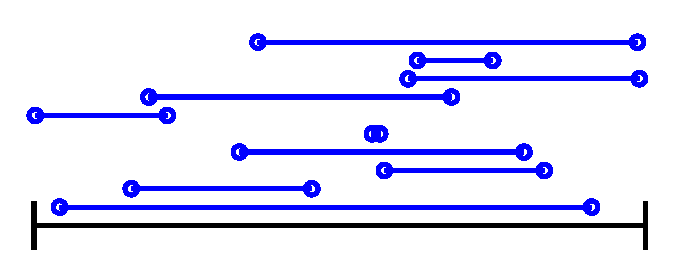
\includegraphics[width=0.35\columnwidth]{../Matlab/Plots/LinePicking_eg_line.eps}}
       \hspace{0.04\columnwidth}
    \subfloat[\label{fig:line_pdf}PDF.]
       {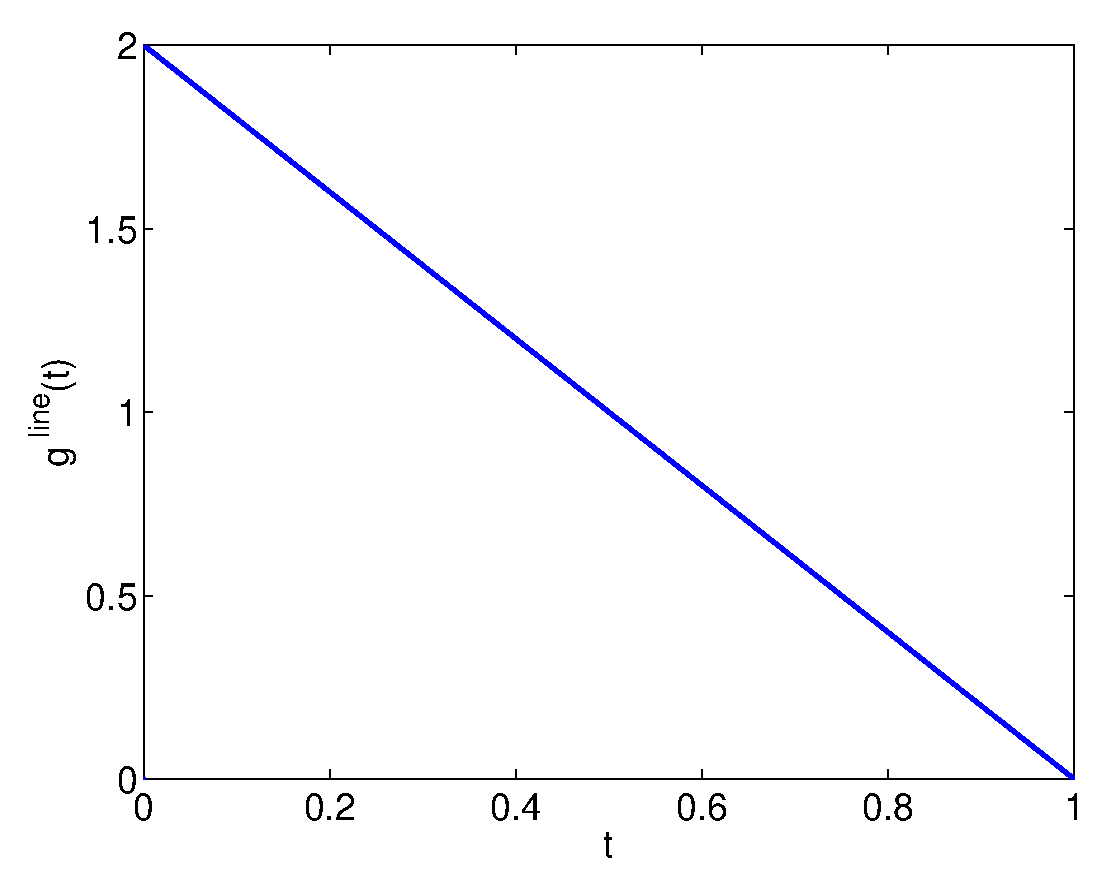
\includegraphics[width=0.6\columnwidth]{../Matlab/Plots/LinePicking_plot_line_pdf.eps}}
    \caption{The line-line picking problem ($L=1$).}
  \end{center}
\vspace{-4mm}
\end{figure}

\begin{table}[ht]
  \centering
  \begin{tabular}{|r|c|l|}
    \hline
    Statistic & Value & Source \\ 
    \hline
      PDF                & $\displaystyle \frac{2}{L} \left( 1-\frac{t}{L} \right)$ &
                             \cite{weisstein:_line_line_picking,b.ghosh51:_random_rect} \\
      CDF                & $\displaystyle \frac{2}{L} t - \frac{t^2}{L^2}$ & 
                             \eqref{eq:line_cdf}\\
      $i$th Moment $m_i$ & $\displaystyle \frac{2 L^{i}}{(i+1)(i+2)}$ &
                             \eqref{eq:line_moments} \\
      Mean               & $\displaystyle \frac{L}{3}$ &
                             \eqref{eq:line_mean} \\
      Variance           & $\displaystyle \frac{L^2}{18}$ &
                             \eqref{eq:line_var} \\[1.5ex]
    \hline
  \end{tabular}
  \caption{Summary of the line-line picking problem for a line of
    length $L$.}
  \label{tab:summary_line}
\end{table}

\subsubsection{PDF}

The probability density function of distances between two (uniformly)
randomly chosen points on the unit line is given in
\cite{weisstein:_line_line_picking,b.ghosh51:_random_rect}, as
$g^{\rm line}(t) = 2(1-t)$, or for a line of length $L$
\begin{equation}
  \label{eq:line_line}
  g^{\rm line}_L(t) = \frac{2}{L} \left( 1-\frac{t}{L} \right).
\end{equation}
This also arises as the limit as $a \rightarrow 0$ for the PDF for the
rectangle \eqref{eqn:rectangle}. 

\subsubsection{CDF}

The CDF can be obtained by simple integration:
\begin{equation}
  \label{eq:line_cdf}
    G^{\rm line}_L(t)
 = \int_0^t g^{\rm line}_L(s) \, ds
 =  \frac{2}{L} t - \frac{t^2}{L^2}. 
\end{equation}
% \begin{eqnarray}
%   G^{\rm line}_L(t)
%      & = & \int_0^t g^{\rm line}_L(s) \, ds, \nonumber \\ 
%      & = & \frac{2}{L} \int_0^t  1-\frac{s}{L} \, ds, \nonumber \\ 
%      & = & \frac{2}{L} \left[ s - \frac{s^2}{2L} \right]_0^t, \nonumber \\ 
%      & = &  \frac{2}{L} t - \frac{t^2}{L^2}.
%   \label{eq:line_cdf}  
% \end{eqnarray}

\subsubsection{Moments}

The moments are also given directly by integration:
\begin{equation}
   \label{eq:line_moments}
   m^{\rm line}_i = \int_0^L s^i g^{\rm line}_L(s) \, ds = \frac{2 L^{i}}{(i+1)(i+2)},
\end{equation}
and the mean and Variance are therefore
\begin{eqnarray}
  \mu^{\rm line} & = & \frac{L}{3},
  \label{eq:line_mean} \\
  \sigma^2_{\rm line}
%       & = & \frac{2 L^{2}}{12} - \frac{L^2}{9}, \nonumber \\
%       & = & \frac{6 L^{2} -4 L^2}{36}, \nonumber \\
      & = & \frac{L^{2}}{18}.
  \label{eq:line_var}
\end{eqnarray}

% \begin{eqnarray}
%   \alpha_i & = & \int_0^L s^i g^{\rm line}_L(s) \, ds, \nonumber \\
%            & = & \frac{2}{L}  \int_0^L s^i- \frac{s^{i+1}}{L}  \, ds, \nonumber \\
%            & = & \frac{2}{L} \left[ \frac{s^{i+1}}{i+1} - \frac{s^{i+2}}{L(i+2)} \right]_0^L, \nonumber \\
%            & = & \frac{2 L^{i}}{i+1} - \frac{2 L^{i}}{(i+2)}, \nonumber \\
%            & = & \frac{2 L^{i} (i+2) - 2 L^{i}(i+1)}{(i+1)(i+2)} , \nonumber \\
%            & = & \frac{2 L^{i}}{(i+1)(i+2)} , \nonumber \\
%   \label{eq:line_moments}
% \end{eqnarray}
% Hence the mean and variance are
% \begin{eqnarray}
%   \mu^{\rm line} & = & \frac{L}{3}, \\
%   \label{eq:line_mean}
%   \sigma^2_{\rm line}
%       & = & \frac{2 L^{2}}{12} - \frac{L^2}{9}, \nonumber \\
%       & = & \frac{6 L^{2} -4 L^2}{36}, \nonumber \\
%       & = & \frac{L^{2}}{18}.
%   \label{eq:line_var}
% \end{eqnarray}


